\section*{* 附錄一\quad 希耳伯特 (Hilbert) 歐氏空間的公理幾何}
\addcontentsline{toc}{section}{* 附錄一\quad 希耳伯特 (Hilbert) 歐氏空間的公理幾何}
\label{sec:b3_a1}

\renewcommand{\thefigure}{附1-\arabic{figure}}
\setcounter{figure}{0}

對於空間有系統的研究，起始於古埃及時代；而在古希臘時代獲得了輝煌的成就。其中集其大成者，也就是數學史上的重要著作——歐幾里德的幾何原理。歐氏幾何原理所採用的體系如下：

它將已往對於空間經由觀察、實驗、研討所得的結果，加以歸納、分析、精鍊而得出空間的一組基本概念與一組基本性質，然後以這一組基本概念為出發點，逐步闡述其他關於空間的概念；以這一組基本性質為基礎，有系統地用邏輯去推演空間的各種其他性質。這裏要談的，大體上就是歐氏幾何原理中所採用的基本概念與基本性質。

我們在第一冊引言裏提過“公理化”的過程。空間既然是我們平日生活所在，我們自然對它收集了大量的經驗事實，把這些經驗事實一一列舉說明，不但極不經濟，不合治學之道，因為事實之間的相互關係，以及那些事實具有特殊重要性，並不能一目瞭然。公理化的用意，即要從大量雜亂無章的經驗事實中，抽出“少量的”，“簡單的”幾個事實作為基本，然後證明其他所有已由經驗得到的事實，不過都是這幾個基本事實的邏輯性必然推論。更重要的是，從這些簡單的，又不失其普遍性的公理，較容易而確切地推知一些未知的，不能全仗經驗充分地建立其確性的事實。

歐氏幾何原理的整個體系，大致上業已相當完備，但是依然有不少欠缺和不夠清晰的地方，到十九世紀末希耳伯特 (D. Hilbert) 將其重新整理而得一較完備的體系。

從方法論的觀點看，公理化的好處在於使一個複雜的體系有一個很清楚的脈絡，可以說是以簡御繁，但希耳伯特公理化幾何的導引過程是數學本身的一支，並不直接有助於實際問題的處理，所以我們把它放在這裏講。

% ==========================================
% § 1 點、直線、平面的相互關係
% ==========================================
\subsection*{\S 1\quad 點、直線、平面的相互關係}
\addcontentsline{toc}{subsection}{\S 1\quad 點、直線、平面的相互關係}
\label{sec:b3_a1_1}

點是用來表現“位置”的，（點只有位置，沒有大小），是空間中“位置”這個概念的抽象；\underline{直線}是用來表現“方向”的，是空間中“方向”這個概念的抽象；我們用一個有向直線來表示空間的一個方向。

\begin{center}
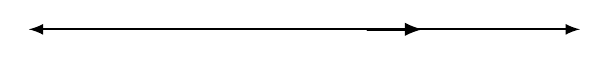
\begin{tikzpicture}[>=latex, line cap=round, line join=round]
  \draw[<->, thick] (-3.5,0) -- (3.5,0);
  \draw[->, very thick] (0.8,0) -- (1.5,0);
\end{tikzpicture}
\end{center}

\noindent\textbf{基本性質 $\mathrm{I}_a$：}任給空間相異兩點 $A, B$，有一條唯一的直線通過這兩點 $A, B$，亦即相異兩點決定一直線。

\noindent\textbf{推論 1}\quad 相異兩直線 $l, m$，假若相交（亦即交集 $l \cap m \neq \phi$）則只交於一點（亦即交集 $l \cap m$ 只含有一個點）。

上述推論是性質 $\mathrm{I}_a$ 的直接結論，因為假如 $l \cap m$ 含有兩個或更多的點，則由性質 $\mathrm{I}_a$ 即得 $l, m$ 是同一條直線，這和 $l, m$ 相異的假設不合。

「平面」是一個到處平直的面，亦即

\noindent\textbf{基本性質 $\mathrm{I}_b$：}過平面上任意兩點的直線完全包含在該平面之內。

\begin{figure}[H]
\centering
\begin{tikzpicture}[>=latex, line cap=round, line join=round, scale=0.9]
  % 平面四邊形
  \draw[thick] (0,0) -- (6.5,0) -- (7.5,2.5) -- (1.0,2.5) -- cycle;
  \node at (7.8,2.2) {\small 平面};

  % 通過 A, B 的直線
  \coordinate (A) at (2.0,0.6);
  \coordinate (B) at (4.8,1.8);
  \draw[<->, thick] ($(A)!-0.4!(B)$) -- ($(A)!1.4!(B)$);
  \filldraw (A) circle (1.5pt) node[above left=1pt] {$A$};
  \filldraw (B) circle (1.5pt) node[above left=1pt] {$B$};

  % 相交直線 CD
  \coordinate (C) at (2.2,2.3);
  \coordinate (D) at (4.2,0.2);
  \draw[<->, thick] ($(C)!-0.2!(D)$) -- ($(C)!1.2!(D)$);
  \filldraw (C) circle (1.5pt) node[above right=1pt] {$C$};
  \filldraw (D) circle (1.5pt) node[below right=1pt] {$D$};
\end{tikzpicture}
\caption{直線與平面}
\label{fig:b3-a1-1}
\end{figure}

\noindent\textbf{推論 2}\quad 對於空間的一個平面 $P$ 和一條直線 $l$，其交集只有下列三種可能：
\begin{enumerate}[(i), leftmargin=2.5em]
  \item $P \cap l = \phi$（空集合），亦即不相交，
  \item $P \cap l$ 只含有一個點，亦即交於一點，
  \item $P \cap l = l$\phantomsection\label{note:b3-a1-p261-order}\footnote{【原書註記/校訂】：原書印作「亦即 $l$ 完全包含 $P$ 在中」，依文義實為「$l$ 完全包含在 $P$ 中」（或「$P$ 完全包含 $l$」）．正文照原印字樣錄入．} 亦即 $l$ 完全包含 $P$ 在中，
\end{enumerate}
\noindent【註】\quad 因為假如 $P \cap l$ 含有兩個或更多的點，由性質 $\mathrm{I}_b$ 可知 $P \cap l = l$。

\noindent\textbf{基本性質 $\mathrm{I}_c$：}過空間不共線三點，有一個唯一的平面。亦即不共線三點決定一平面。

\begin{figure}[H]
\centering
\begin{tikzpicture}[>=latex, line cap=round, line join=round, scale=0.9]
  % 平面 P (傾斜)
  \draw[thick, fill=gray!25] (1.0,0.5) -- (5.5,0.5) -- (6.5,4.0) -- (2.0,4.0) -- cycle;
  \node at (6.8,3.8) {\small 平面 $\mathbf{P}$};

  % 平面 Q (橫向穿過)
  \draw[thick, fill=gray!10, fill opacity=0.8] (0.0,2.5) -- (5.5,1.5) -- (7.5,1.5) -- (2.0,2.5) -- cycle;
  \node at (7.8,1.3) {\small 平面 $\mathbf{Q}$};

  % 交線 AB
  \coordinate (A) at (1.8,2.15);
  \coordinate (B) at (4.7,1.65);
  \draw[very thick] ($(A)!-0.3!(B)$) -- ($(A)!1.3!(B)$);
  \draw[dashed, thick] ($(A)!1.3!(B)$) -- ($(A)!1.6!(B)$);
  \draw[dashed, thick] ($(A)!-0.3!(B)$) -- ($(A)!-0.6!(B)$);

  \filldraw (A) circle (1.5pt) node[above=2pt] {$A$};
  \filldraw (B) circle (1.5pt) node[above=2pt] {$B$};

  \coordinate (C) at (3.8,3.8);
  \filldraw (C) circle (1.5pt) node[right=2pt] {$C$};

  \coordinate (D) at (5.8,1.4);
  \filldraw (D) circle (1.5pt) node[above=2pt] {$D$};
\end{tikzpicture}
\caption{兩平面之相交}
\label{fig:b3-a1-2}
\end{figure}

\noindent\textbf{基本性質 $\mathrm{I}_d$：}相異兩平面若相交則交集為一直線。

如圖 \ref{fig:b3-a1-2} 所示，$A, B, C$ 三點不共線，決定平面 $P$，$A, B, D$ 三點不共線，決定平面 $Q$，平面 $P$ 與平面 $Q$ 交於一直線，即過 $A, B$ 的直線。

\noindent\textbf{基本性質 $\mathrm{I}_e$：}一直線上至少有兩點；一平面上至少有不共線的三點；空間至少有不共面的四點。

以上基本性質 $\mathrm{I}_a \sim \mathrm{I}_e$ 已提供了空間的結構。

\subsection*{習題 1}
\begin{enumerate}[1., leftmargin=2em]
  \item 若把基本性質 $\mathrm{I}_d$ 改成：
  \begin{quote}
    $\mathrm{I}_d'$：相異兩平面若相交，則交點至少有兩個。
  \end{quote}
  試證：$\mathrm{I}_d$ 可以由 $\mathrm{I}_b, \mathrm{I}_c$ 及 $\mathrm{I}_d'$ 導出，\\
  就是說：性質 $\mathrm{I}_d'$ 較弱，但可以取代 $\mathrm{I}_d$。
\end{enumerate}

% ==========================================
% § 2 次序與分隔
% ==========================================
\subsection*{\S 2\quad 次序與分隔}
\addcontentsline{toc}{subsection}{\S 2\quad 次序與分隔}
\label{sec:b3_a1_2}

\subsubsection*{甲、在第二冊第三章討論實數系的次序關係時}

我們曾提及直線上一點與點之間的次序關係。直線上的次序關係和下列「一目瞭然」的幾何事實密切的關連。
\begin{enumerate}[(i), leftmargin=2.5em]
  \item 直線上一點將該直線分割成兩段。
  \item 平面上的一條直線將該平面分割成兩片。
  \item 空間的一個平面將空間分割成兩部分。
\end{enumerate}

\begin{figure}[H]
\centering
\begin{subfigure}[b]{0.45\textwidth}
\centering
\begin{tikzpicture}[>=latex, scale=0.85]
  \draw[<->, thick] (-2.5,0) -- (2.5,0);
  \filldraw (0,0) circle (2pt) node[above=3pt] {$A$};
  \node at (1.8,-0.6) {\small 刀片割線圖};
\end{tikzpicture}
\caption{3-(i)}
\label{fig:b3-a1-3-1}
\end{subfigure}
\hfill
\begin{subfigure}[b]{0.45\textwidth}
\centering
\begin{tikzpicture}[>=latex, scale=0.85]
  \draw[thick, fill=gray!20] (0,0) -- (4,0) -- (4.8,2.2) -- (0.8,2.2) -- cycle;
  \draw[dashed, thick] (1.5,1.8) -- (3.2,0.3);
  \draw[->, very thick] (2.2,2.4) -- (2.0,1.2);
  \node at (3.8,-0.4) {\small 劈刀剪紙圖};
\end{tikzpicture}
\caption{3-(ii)}
\label{fig:b3-a1-3-2}
\end{subfigure}
\caption{分隔的直觀概念}
\label{fig:b3-a1-3}
\end{figure}

用來描述直線上相異三點相互之間的次序關係的基本術語是：「某一\phantomsection\label{note:b3-a1-p263-point}\footnote{【原書註記/校訂】：原書印作「某一黠位於其餘兩點之間」，「黠」顯為「點」字之字模破殘或印刷油墨污損．正文照原印字樣錄入．}黠位於其餘兩點之間」。

\noindent\textbf{基本性質 $\mathrm{II}_a$：}對於直線上任給相異三點，其中必定有一個唯一的點，它位於其餘兩點之間。

如圖 \ref{fig:b3-a1-4} 所示，直線 $l$ 上三點 $A, B, C$ 的次序關係是：
\begin{quote}
  「$B$ 點位於 $A, C$ 之間」。
\end{quote}

\begin{figure}[H]
\centering
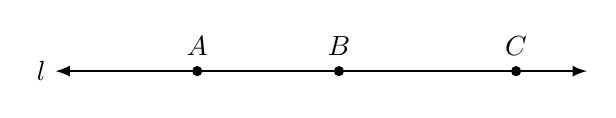
\begin{tikzpicture}[>=latex, scale=0.9]
  \draw[<->, thick] (-1,0) -- (6.5,0);
  \node[left] at (-1,0) {$l$};
  \filldraw (1,0) circle (1.8pt) node[above=2pt] {$A$};
  \filldraw (3,0) circle (1.8pt) node[above=2pt] {$B$};
  \filldraw (5.5,0) circle (1.8pt) node[above=2pt] {$C$};
\end{tikzpicture}
\caption{直線上三點的次序}
\label{fig:b3-a1-4}
\end{figure}

\noindent\textbf{基本性質 $\mathrm{II}_b$：}若 $B$ 點位於 $A, C$ 之間，則 $B$ 點也位於 $C, A$ 之間。換句話說：「位於某兩點之間」這一關係和那兩點的順序無關。

\noindent\textbf{基本性質 $\mathrm{II}_c$：}對於直線上任給相異二點 $A, B$，必定存在有位於 $A, B$ 之間的點（如圖 5(i) 所示）又存在 $D$ 點及 $E$ 點，使得 $B$ 位於 $A, D$ 之間而 $A$ 位於 $B, E$ 之間。

\begin{figure}[H]
\centering
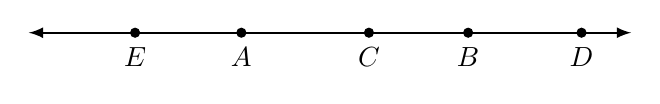
\begin{tikzpicture}[>=latex, scale=0.9]
  \draw[<->, thick] (-1,0) -- (7.5,0);
  \filldraw (0.5,0) circle (1.8pt) node[below=2pt] {$E$};
  \filldraw (2.0,0) circle (1.8pt) node[below=2pt] {$A$};
  \filldraw (3.8,0) circle (1.8pt) node[below=2pt] {$C$};
  \filldraw (5.2,0) circle (1.8pt) node[below=2pt] {$B$};
  \filldraw (6.8,0) circle (1.8pt) node[below=2pt] {$D$};
\end{tikzpicture}
\caption{直線上相異點的存在性}
\label{fig:b3-a1-5-1}
\end{figure}

\noindent\textbf{定義}\quad 由空間的兩點 $\{A, B\}$ 以及「在直線 $AB$ 上所有位於 $A, B$ 之間的點」所成的集合叫做「線段 $AB$」。我們將以符號「$\overline{AB}$」表示「線段 $AB$」（如圖 \ref{fig:b3-a1-6} 的實線部分就是 $\overline{AB}$）。

\begin{figure}[H]
\centering
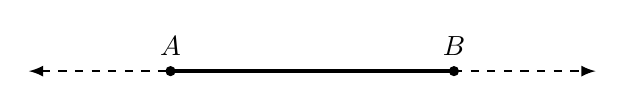
\begin{tikzpicture}[>=latex, scale=0.9]
  \draw[<-, dashed, thick] (-1.5,0) -- (0.5,0);
  \draw[very thick] (0.5,0) -- (4.5,0);
  \draw[->, dashed, thick] (4.5,0) -- (6.5,0);
  \filldraw (0.5,0) circle (1.8pt) node[above=2pt] {$A$};
  \filldraw (4.5,0) circle (1.8pt) node[above=2pt] {$B$};
\end{tikzpicture}
\caption{線段 $\overline{AB}$}
\label{fig:b3-a1-6}
\end{figure}

\subsubsection*{乙、分隔與次序之間的關係}

首先，我們得把直線、平面、空間的「分隔」再說明一下。
\begin{enumerate}[(i), leftmargin=2.5em]
  \item \textbf{直線的分隔：}直線 $l$ 上的一點 $D$，把直線 $l$ 上所有其他的點分隔成兩部分（或兩側），使得屬於同一部分的任意兩點所決定的線段不含 $D$ 點（如圖 5(ii) 的 $B$ 與 $C$；線段 $\overline{BC}$ 不含 $D$ 點）而分別屬於不同部分的任意兩點所決定的線段必含有 $D$ 點（如圖 5(ii) 之 $\overline{AC}$ 與 $\overline{AB}$）。

  \begin{figure}[H]
  \centering
  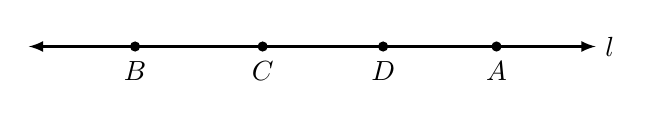
\begin{tikzpicture}[>=latex, scale=0.9]
    \draw[<->, thick] (-1,0) -- (7,0);
    \node[right] at (7,0) {$l$};
    \filldraw (0.5,0) circle (1.8pt) node[below=2pt] {$B$};
    \filldraw (2.3,0) circle (1.8pt) node[below=2pt] {$C$};
    \filldraw (4.0,0) circle (1.8pt) node[below=2pt] {$D$};
    \filldraw (5.6,0) circle (1.8pt) node[below=2pt] {$A$};
  \end{tikzpicture}
  \caption{直線的分隔}
  \label{fig:b3-a1-5-2}
  \end{figure}

  \item \textbf{平面的分隔：}平面 $P$ 上的一條直線 $d$，把平面 $P$ 上所有其他的點分隔成兩部分（或兩側）；使得屬於同一部分的任意兩點所決定的線段和直線 $d$ 不相交（如圖 \ref{fig:b3-a1-7} 中 $BC$），而分別屬於不同部分的任意兩點所決定的線段則必定和直線 $d$ 相交（如同圖 \ref{fig:b3-a1-7} 中 $AB, AC$）。

  \begin{figure}[H]
  \centering
  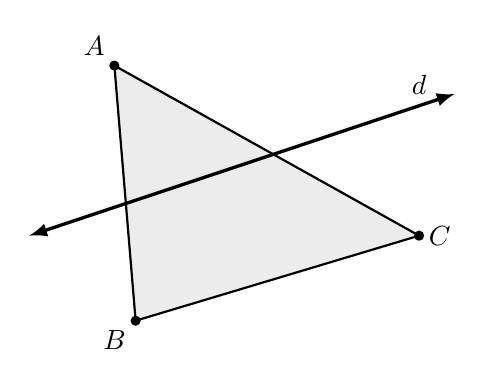
\begin{tikzpicture}[>=latex, scale=0.9]
    \draw[thick, fill=gray!15] (1.2,1.8) -- (1.5,-1.8) -- (5.5,-0.6) -- cycle;
    \filldraw (1.2,1.8) circle (1.8pt) node[above left] {$A$};
    \filldraw (1.5,-1.8) circle (1.8pt) node[below left] {$B$};
    \filldraw (5.5,-0.6) circle (1.8pt) node[right] {$C$};

    \draw[<->, very thick] (0,-0.6) -- (6,1.4);
    \node[above] at (5.5,1.25) {$d$};
  \end{tikzpicture}
  \caption{平面的分隔}
  \label{fig:b3-a1-7}
  \end{figure}

  \item \textbf{空間的分隔：}一個平面 $D$，把空間所有不在 $D$ 上的點分成兩部分（或兩側）；使得屬於同一部分（或同側）的任意兩點所決定的線段和 $D$ 不相交，而分別屬於不同部分（或異側）的任意兩點所決定的線段必定和 $D$ 相交。

  \begin{figure}[H]
  \centering
  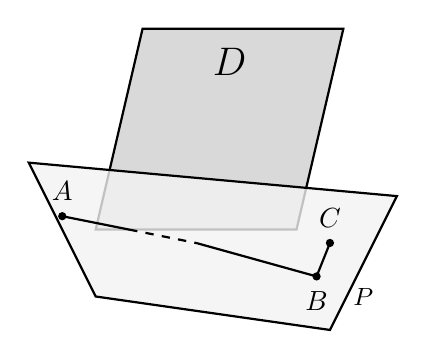
\begin{tikzpicture}[>=latex, scale=0.85]
    % 垂直平面 D
    \draw[thick, fill=gray!30] (1.5,1.0) -- (4.5,1.0) -- (5.2,4.0) -- (2.2,4.0) -- cycle;
    \node at (3.5,3.5) {\Large $\mathscr{D}$};

    % 傾斜平面 P
    \draw[thick, fill=gray!10, fill opacity=0.8] (0.5,2.0) -- (6.0,1.5) -- (5.0,-0.5) -- (1.5,0.0) -- cycle;
    \node at (5.5,0.0) {\small $P$};

    % 交線與點
    \coordinate (A) at (1.0,1.2);
    \coordinate (B) at (4.8,0.3);
    \coordinate (C) at (5.0,0.8);
    \filldraw (A) circle (1.5pt) node[above=2pt] {$A$};
    \filldraw (B) circle (1.5pt) node[below=2pt] {$B$};
    \filldraw (C) circle (1.5pt) node[above=2pt] {$C$};
    \draw[thick] (A) -- (2.0,1.0);
    \draw[dashed, thick] (2.0,1.0) -- (3.0,0.8);
    \draw[thick] (3.0,0.8) -- (B);
    \draw[thick] (B) -- (C);
  \end{tikzpicture}
  \caption{空間的分隔}
  \label{fig:b3-a1-8}
  \end{figure}
\end{enumerate}

其次我們要來分析一下上述三種「分隔」相互之間的關係：
\begin{enumerate}[(1), leftmargin=2em]
  \item 當圖 5(ii) 中的 $A, B, C$ 三點是在一條直線 $l$ 上，亦即三點共線時，（稱 $l$ 和 $d$ 的交點為 $D$），則圖 5 包含在圖 7 之中，所以當我們把「平面的分隔」局限到一條和 $d$ 相交的直線 $l$ 上，即得「直線的分隔」，換句話說：「直線的分隔」是「平面的分隔」的一個特殊情形。
  \item 假如我們把圖 \ref{fig:b3-a1-8} 中過 $A, B, C$ 的平面叫做 $P$，平面 $D$ 和 $P$ 的交線叫做 $d$，則圖 \ref{fig:b3-a1-8} 局限在 $P$ 的部分就是圖 \ref{fig:b3-a1-7}。所以對於空間任意三點的分隔乃是「平面分隔」的直接推論（因為空間任意三點皆共面，再者，由對於空間任意三點的分隔我們容易推演得 (iii) 中所述的「空間的分隔」（參看以下對平面情形的討論），這就說明了空間的分隔是平面的分隔的一個直接推論。）
\end{enumerate}

由上面的解說，我們知道關於直線、平面、空間這三種情形的分隔都可以歸於「平面的分隔」這一種情形來討論。我們把「平面上任意三點的分隔」重述如下：（參看圖 \ref{fig:b3-a1-7}）

平面 $P$ 上的一直線 $d$，把平面 $P$ 上所有其他的點分隔成兩部分（或兩側）；使得屬於同一部分兩點所決定的線段和直線 $d$ 不相交，而分別屬於不同部分\phantomsection\label{note:b3-a1-p266-de}\footnote{【原書註記/校訂】：原書印作「而分別屬於不同部分得兩點所決定的線段」，「得」實為助詞「的」之排印訛字．正文照原印字樣錄入．}得兩點所決定的線段則必定和直線 $d$ 相交。

\noindent\textbf{推論 3}\quad 同在平面 $P$ 上的 $\triangle ABC$ 和直線 $d$，若 $A, B, C$ 皆不在 $d$ 上，而且 $d$ 和 $AB$ 交於一點；則 $d$ 必定和 $BC, AC$ 這個線段中的一個而且只有一個相交（註）。

\begin{figure}[H]
\centering
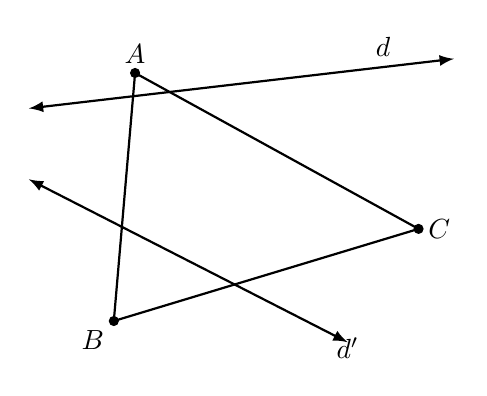
\begin{tikzpicture}[>=latex, scale=0.9]
  \coordinate (A) at (1.5,2.0);
  \coordinate (B) at (1.2,-1.5);
  \coordinate (C) at (5.5,-0.2);

  \draw[thick] (A) -- (B) -- (C) -- cycle;
  \filldraw (A) circle (1.8pt) node[above] {$A$};
  \filldraw (B) circle (1.8pt) node[below left] {$B$};
  \filldraw (C) circle (1.8pt) node[right] {$C$};

  % 直線 d (交 AB 與 AC)
  \draw[<->, thick] (0.0,1.5) -- (6.0,2.2);
  \node[above] at (5.0,2.1) {$d$};

  % 直線 d' (交 AB 與 BC)
  \draw[<->, thick] (0.0,0.5) -- (4.5,-1.8);
  \node[below] at (4.5,-1.6) {$d'$};
\end{tikzpicture}
\caption{推論 3 示意圖}
\label{fig:b3-a1-9}
\end{figure}

\noindent\textbf{推論 4}\quad 同在平面 $P$ 上的 $\triangle ABC$ 和直線 $d$。若 $A, B, C$ 皆不在 $d$ 上而且 $d$ 和 $BC, AC$ 不相交，則 $d$ 和 $AB$ 也不相交。

\noindent\textbf{推論 5}\quad 如圖 \ref{fig:b3-a1-10} 所示，直線 $d$ 和 $\triangle ABC$ 的兩邊 $AB, AC$ 相交，而和 $BC$ 不相交。設 $C'$ 是另外一個不在直線 $d$ 上的點，而且 $CC'$ 和 $d$ 不相交，則必有 $BC'$ 和 $d$ 不相交而 $AC'$ 和 $d$ 相交。

\noindent【註】\quad $A, B, C$ 不在 $d$ 上，而且 $\overline{AB}$ 和 $d$ 相交，所以 $A, B$ 兩點分別位於 $d$ 的不同兩側，假如 $C$ 點和 $A$ 同側則必和 $B$ 異側，亦即 $d$ 和 $\overline{BC}$ 相交，但是和 $\overline{AC}$ 不相交，假如 $C$ 點和 $B$ 同側必和 $A$ 異側，亦即 $d$ 和 $\overline{AC}$ 相交，但是和 $\overline{BC}$ 不相交。

\begin{figure}[H]
\centering
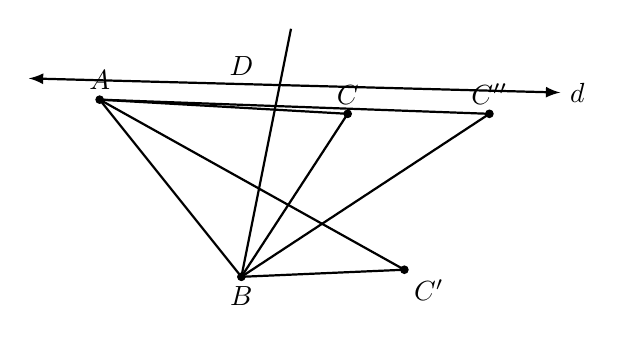
\begin{tikzpicture}[>=latex, scale=0.9]
  \coordinate (A) at (1.5,2.0);
  \coordinate (B) at (3.5,-0.5);
  \coordinate (C) at (5.0,1.8);
  \coordinate (Cp) at (5.8,-0.4);
  \coordinate (Cpp) at (7.0,1.8);

  \draw[thick] (A) -- (B) -- (C) -- cycle;
  \draw[thick] (B) -- (Cp) -- (A);
  \draw[thick] (B) -- (Cpp) -- (A);

  % 頂點標記
  \filldraw (A) circle (1.5pt) node[above] {$A$};
  \filldraw (B) circle (1.5pt) node[below] {$B$};
  \filldraw (C) circle (1.5pt) node[above] {$C$};
  \filldraw (Cp) circle (1.5pt) node[below right] {$C'$};
  \filldraw (Cpp) circle (1.5pt) node[above] {$C''$};

  % 直線 d
  \draw[<->, thick] (0.5,2.3) -- (8.0,2.1);
  \node[right] at (8.0,2.1) {$d$};

  % 交點 D
  \coordinate (D) at (3.5,2.2);
  \node[above] at (D) {$D$};
  \draw[thick] (B) -- (4.2,3.0);
\end{tikzpicture}
\caption{推論 5 與推論 6 示意圖}
\label{fig:b3-a1-10}
\end{figure}

\noindent【證明】\quad 推論 4 是推論 3 的直接結論，至於推論 5 由 $BC, CC'$ 和 $d$ 不相交及推論 4 可知 $BC'$ 和 $d$ 也不相交，再由推論 3（用在 $\triangle ABC'$ 或 $ACC'$ 上）即得 $AC'$ 和 $d$ 必定相交。

當 $C'$ 點在 $AC$ 連線 $l$ 上時（如圖 \ref{fig:b3-a1-10} 所示的 $C'$）即得直線 $l$ 上 $A, C, C'$ 三點的分隔。

\noindent\textbf{推論 6}\quad 直線上四點 $A, D, C, C''$ 之間的關係若為 $D$ 位於 $A, C$ 之間，而且 $D$ 不在 $C, C''$ 之間，則必定有關係：$D$ 位於 $A, C''$ 之間。

\noindent【證明】\quad 這是在推論 5 中當 $C''$ 點和 $A, D$ 共線的特殊情形。

\noindent\textbf{推論 7}\quad 直線上四點 $A, B, C, D$ 之間的關係若為：
\begin{quote}
  $B$ 位於 $A$ 與 $C$ 之間，而且 $C$ 位於 $B$ 與 $D$ 之間，則必定也有關係：$B$ 位於 $A$ 與 $D$ 之間和 $C$ 位於 $A$ 與 $D$ 之間。
\end{quote}

\noindent【證明】\quad
\begin{align*}
  &\text{「$B$ 位於 $A$ 與 $C$ 之間」而且「$C$ 位於 $B$ 與 $D$ 之間」（性質 $\mathrm{II}_a$）} \\
  &\Downarrow \\
  &\text{「$B$ 位於 $A$ 與 $C$ 之間」而且「$B$ 不在 $C$ 與 $D$ 之間」（推論 5；將 $B$ 換 $D, D$ 換 $C''$。）} \\
  &\Downarrow \\
  &\text{「$B$ 位於 $A$ 與 $D$ 之間」}
\end{align*}
再者，由性質 $\mathrm{II}_b$ 知道「位於某某之間」這種關係是對稱的，亦即
\begin{align*}
  &\text{「$B$ 位於 $A$ 與 $C$ 之間」和「$C$ 位於 $B$ 與 $D$ 之間」} \\
  &\Updownarrow \\
  &\text{「$C$ 位於 $D$ 與 $B$ 之間」和「$B$ 位於 $C$ 與 $A$ 之間」}
\end{align*}
所以只要把 $A$ 與 $D$ 互換，$B$ 與 $C$ 互換，同理可證出「$C$ 位於 $D$ 與 $A$ 之間」（$\Longleftrightarrow$「$C$ 位於 $A$ 與 $D$ 之間」）。

\begin{figure}[H]
\centering
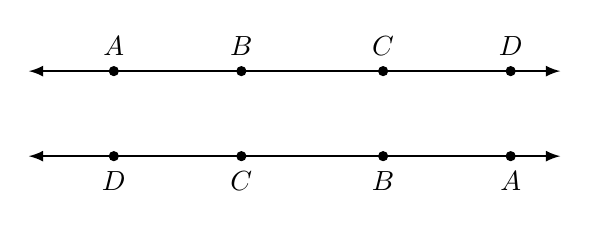
\begin{tikzpicture}[>=latex, scale=0.9]
  % 上軸
  \draw[<->, thick] (0,1.2) -- (7.5,1.2);
  \filldraw (1.2,1.2) circle (1.8pt) node[above=2pt] {$A$};
  \filldraw (3.0,1.2) circle (1.8pt) node[above=2pt] {$B$};
  \filldraw (5.0,1.2) circle (1.8pt) node[above=2pt] {$C$};
  \filldraw (6.8,1.2) circle (1.8pt) node[above=2pt] {$D$};

  % 下軸
  \draw[<->, thick] (0,0) -- (7.5,0);
  \filldraw (1.2,0) circle (1.8pt) node[below=2pt] {$D$};
  \filldraw (3.0,0) circle (1.8pt) node[below=2pt] {$C$};
  \filldraw (5.0,0) circle (1.8pt) node[below=2pt] {$B$};
  \filldraw (6.8,0) circle (1.8pt) node[below=2pt] {$A$};
\end{tikzpicture}
\caption{直線上四點次序之對稱性}
\label{fig:b3-a1-11}
\end{figure}

\subsection*{習題 2}
\begin{enumerate}[1., leftmargin=2em]
  \item 討論直線上任意四點的次序關係，試證在適當的調整各點名稱後其次序關係為 $ABCD$ 亦即
  \[
  \begin{cases}
    B \text{ 位於 } AC \text{ 之間}, & B \text{ 位於 } AD \text{ 之間} \\
    C \text{ 位於 } BD \text{ 之間}, & C \text{ 位於 } AD \text{ 之間}
  \end{cases}
  \quad \text{同時成立。}
  \]
  \item 討論直線上任意五點的次序關係。
\end{enumerate}

% ==========================================
% § 3 空間的均勻性與疊合關係（全等關係）
% ==========================================
\subsection*{\S 3\quad 空間的均勻性與疊合關係（全等關係）}
\addcontentsline{toc}{subsection}{\S 3\quad 空間的均勻性與疊合關係（全等關係）}
\label{sec:b3_a1_3}

\subsubsection*{甲、均勻與到處相同}

在討論空間的均勻性之前，讓我們先\phantomsection\label{note:b3-a1-p268-xian}\footnote{【原書註記/校訂】：原書印作「讓我們先生舉幾個淺顯常見的例子」，多印一「生」字，實為「先舉」．正文照原印字樣錄入．}生舉幾個淺顯常見的例子來說明均勻性這個觀念，譬如當你油漆一面牆壁時，你就得要注意色澤深淺是否均勻。當你把一滴紅墨水滴到一瓶清水裏，剛開始是非常不均勻的，但是由於逐漸的擴散作用，經過相當一段時間後就變成一瓶均勻的淡紅色溶液，在上面兩個例子中，「均勻」的意思可以解釋成「到處相同」，在這裏「空間的均勻性」要指的也是：
\begin{quote}
  「空間是均勻而到處相同的這個基本性質。」
\end{quote}

我們在所生活的鄰近，經由觀察、實驗、研討，可以得到很多有用的幾何性質，但是這只是我們所在鄰近的幾何性質，是不是這些「我們的鄰近所有的幾何性質」在另外一個遙遠的星球上依然成立呢？這是個很耐人尋味的問題，在我們步履可及的部分，空間的均勻性是可以由實驗與經驗加以證實的。至於那些太空遙遠的角落，是不是真的和我們所在的鄰近具有同樣的幾何性質？不身歷其「境」是無法解答的，所以嚴格的說來，「空間的均勻性乃是一個大膽的假設」，我們所以敢作這樣大膽的假設是因為：至少在我們可能驗證的範圍之內，亦即在地球上，假設地球是個正球體不是扁的，或橢圓體，空間是均勻的，但並不是所有空間都是均勻的，如圖 \ref{fig:b3-a1-12} 所示。不均勻的救生圈面（環面）。$AC = A'C', AB = A'B', \angle BAC = \angle B'A'C' = 90^\circ$，但 $\triangle ABC$ 與 $\triangle A'B'C'$ 不全等。

\begin{figure}[H]
\centering
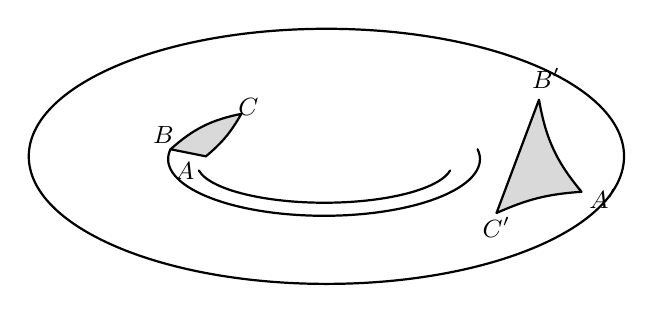
\begin{tikzpicture}[scale=0.9, line cap=round, line join=round]
  % 環面外輪廓
  \draw[thick] (0,0) ellipse (4.2cm and 1.8cm);

  % 環面內孔
  \draw[thick] (-2.2,0.1) arc (170:370:2.2cm and 0.8cm);
  \draw[thick] (-1.8,-0.2) arc (-170:-10:1.8cm and 0.55cm);

  % 內側鞍狀三角形 ABC
  \draw[thick, fill=gray!30] (-2.2,0.1) to[bend left=15] (-1.2,0.6) to[bend left=10] (-1.7,0.0) -- cycle;
  \node at (-2.3,0.3) {\small $B$};
  \node at (-1.1,0.7) {\small $C$};
  \node at (-2.0,-0.2) {\small $A$};

  % 外側凸狀三角形 A'B'C'
  \draw[thick, fill=gray!30] (3.0,0.8) to[bend right=15] (3.6,-0.5) to[bend right=10] (2.4,-0.8) -- cycle;
  \node at (3.1,1.1) {\small $B'$};
  \node at (3.9,-0.6) {\small $A'$};
  \node at (2.4,-1.0) {\small $C'$};
\end{tikzpicture}
\caption{不均勻曲面（環面）上之幾何形狀}
\label{fig:b3-a1-12}
\end{figure}

\subsubsection*{乙、均勻性與疊合關係（或全等關係）}

設 $\varGamma, \varGamma'$ 是空間的兩個幾何圖形。假如 $\varGamma$ 和 $\varGamma'$ 的形狀大小完全一樣，我們就說 $\varGamma$ 和 $\varGamma'$ 全等，以符號 $\varGamma \cong \varGamma'$ 記之。

以兩三角形 $\triangle ABC$ 和 $\triangle A'B'C'$ 為例。假如它們的三個邊和三個角對應相等，則 $\triangle ABC$ 和 $\triangle A'B'C'$ 全等。

\begin{figure}[H]
\centering
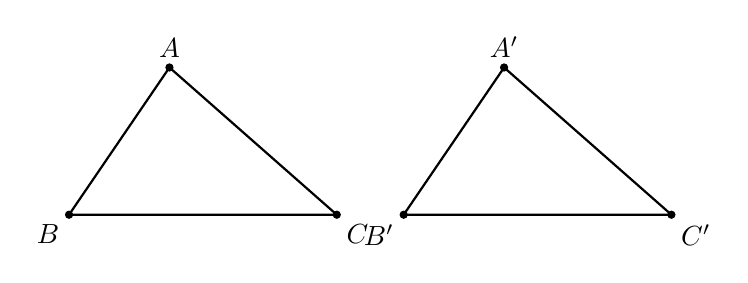
\begin{tikzpicture}[>=latex, scale=0.85]
  % 左三角形 ABC
  \coordinate (A) at (1.5,2.2);
  \coordinate (B) at (0,0);
  \coordinate (C) at (4.0,0);
  \draw[thick] (A) -- (B) -- (C) -- cycle;
  \filldraw (A) circle (1.5pt) node[above] {$A$};
  \filldraw (B) circle (1.5pt) node[below left] {$B$};
  \filldraw (C) circle (1.5pt) node[below right] {$C$};

  % 右三角形 A'B'C'
  \coordinate (Ap) at (6.5,2.2);
  \coordinate (Bp) at (5.0,0);
  \coordinate (Cp) at (9.0,0);
  \draw[thick] (Ap) -- (Bp) -- (Cp) -- cycle;
  \filldraw (Ap) circle (1.5pt) node[above] {$A'$};
  \filldraw (Bp) circle (1.5pt) node[below left] {$B'$};
  \filldraw (Cp) circle (1.5pt) node[below right] {$C'$};
\end{tikzpicture}
\caption{全等三角形}
\label{fig:b3-a1-13}
\end{figure}

一般說來，假如圖形 $\varGamma$ 能夠搬到 $\varGamma'$ 處和 $\varGamma'$ 完全疊合，則 $\varGamma$ 和 $\varGamma'$ 的形狀大小顯然完全一樣，亦即全等。疊合是驗證兩個圖形是否全等的一個直截了當的辦法，所以我們也把全等關係叫做疊合關係。

設 $A, A'$ 為空間任意兩點，空間的均勻性所指的是：空間在 $A$ 點鄰近的部分和其在 $A'$ 點鄰近的部分應該具有相同的幾何性質。我們把上述事實的內涵敘述成下列簡潔的基本形式：

\noindent\textbf{基本性質 $\mathrm{III}_a$：}對於任給線段 $\overline{AB}$ 和過 $A'$ 點的直線 $l'$，在 $l'$ 上 $A'$ 點的兩側分別存在唯一的點 $B', B''$，使得 $\overline{A'B'}$ 及 $\overline{A'B''}$ 和 $\overline{AB}$ 全等（亦即 $\overline{AB}, \overline{A'B'}, \overline{A'B''}$ 等長）。

\begin{figure}[H]
\centering
\begin{tikzpicture}[>=latex, scale=0.9]
  % 線段 AB
  \draw[thick] (-1.0,0) -- (1.0,0);
  \filldraw (-1.0,0) circle (1.8pt) node[above=2pt] {$A$};
  \filldraw (1.0,0) circle (1.8pt) node[above=2pt] {$B$};

  % 直線 l'
  \draw[<->, thick] (1.0,2.5) -- (6.0,-2.0);
  \coordinate (Ap) at (3.5,0.25);
  \filldraw (Ap) circle (1.8pt) node[above right=2pt] {$A'$};

  \coordinate (Bpp) at ($(Ap)!0.6!(1.0,2.5)$);
  \filldraw (Bpp) circle (1.8pt) node[above right=2pt] {$B''$};

  \coordinate (Bp) at ($(Ap)!0.6!(6.0,-2.0)$);
  \filldraw (Bp) circle (1.8pt) node[above right=2pt] {$B'$};
\end{tikzpicture}
\caption{線段之疊合性質}
\label{fig:b3-a1-14}
\end{figure}

\noindent\textbf{基本性質 $\mathrm{III}_b$：}對於任給 $A$ 點的角 $(l_1, l_2)$ 以及任給過另一點 $A'$ 點的平面 $P'$ 和 $P'$ 上的一（有向）直線 $l_1'$，則在 $P'$ 上直線 $l_1'$ 的兩側分別存在唯一的過 $A'$ 點（有向）直線 $l_2'$ 和 $l_2''$ 使得角 $(l_1', l_2')$ 和角 $(l_1, l_2)$ 全等〔亦即角 $(l_1', l_2')$，角 $(l_1', l_2'')$ 和角 $(l_1, l_2)$ 的角度相等。〕

\begin{figure}[H]
\centering
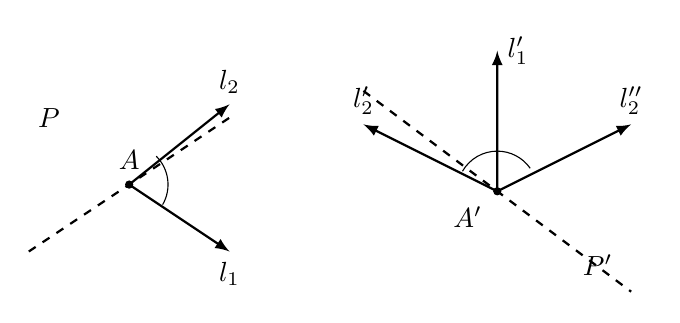
\begin{tikzpicture}[>=latex, scale=0.85]
  % 平面 P 上的角
  \draw[dashed, thick] (-3.5,-1.2) -- (-0.5,0.8);
  \coordinate (A) at (-2.0,-0.2);
  \filldraw (A) circle (1.5pt) node[above=2pt] {$A$};
  \node at (-3.2,0.8) {$P$};
  \draw[->, thick] (A) -- (-0.5,1.0) node[above] {$l_2$};
  \draw[->, thick] (A) -- (-0.5,-1.2) node[below] {$l_1$};
  \draw (-1.5,-0.5) arc (-30:45:0.6);

  % 平面 P' 上的角
  \draw[dashed, thick] (1.5,1.2) -- (5.5,-1.8);
  \coordinate (Ap) at (3.5,-0.3);
  \filldraw (Ap) circle (1.5pt) node[below left=2pt] {$A'$};
  \node at (5.0,-1.4) {$P'$};
  \draw[->, thick] (Ap) -- (3.5,1.8) node[right] {$l_1'$};
  \draw[->, thick] (Ap) -- (1.5,0.7) node[above] {$l_2'$};
  \draw[->, thick] (Ap) -- (5.5,0.7) node[above] {$l_2''$};
  \draw (3.5,0.3) arc (90:150:0.6);
  \draw (3.5,0.3) arc (90:35:0.6);
\end{tikzpicture}
\caption{角之疊合性質}
\label{fig:b3-a1-15}
\end{figure}

\noindent\textbf{基本性質 $\mathrm{III}_c$：}$\triangle ABC$ 和 $\triangle A'B'C'$ 若有
\[ \angle A = \angle A', \quad \overline{AB} = \overline{A'B'}, \quad \overline{AC} = \overline{A'C'} \]
則 $\triangle ABC$ 和 $\triangle A'B'C'$ 能互相疊合（亦即全等），故必然也有
\[ \angle B = \angle B', \quad \angle C = \angle C' \quad \text{及} \quad \overline{BC} = \overline{B'C'} \text{。} \]

\begin{figure}[H]
\centering
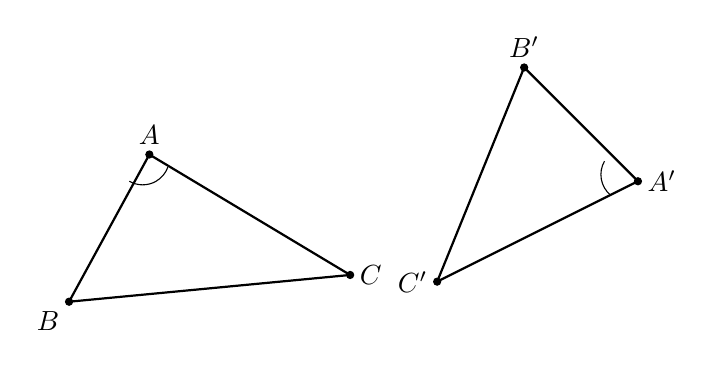
\begin{tikzpicture}[>=latex, scale=0.85]
  % 左三角形 ABC
  \coordinate (A) at (1.2,2.2);
  \coordinate (B) at (0,0);
  \coordinate (C) at (4.2,0.4);
  \draw[thick] (A) -- (B) -- (C) -- cycle;
  \filldraw (A) circle (1.5pt) node[above] {$A$};
  \filldraw (B) circle (1.5pt) node[below left] {$B$};
  \filldraw (C) circle (1.5pt) node[right] {$C$};
  \draw (0.9,1.8) arc (-120:-20:0.4);

  % 右三角形 A'B'C'
  \coordinate (Ap) at (8.5,1.8);
  \coordinate (Bp) at (6.8,3.5);
  \coordinate (Cp) at (5.5,0.3);
  \draw[thick] (Ap) -- (Bp) -- (Cp) -- cycle;
  \filldraw (Ap) circle (1.5pt) node[right] {$A'$};
  \filldraw (Bp) circle (1.5pt) node[above] {$B'$};
  \filldraw (Cp) circle (1.5pt) node[left] {$C'$};
  \draw (8.0,2.1) arc (150:230:0.4);
\end{tikzpicture}
\caption{三角形之邊角疊合 (SAS)}
\label{fig:b3-a1-16}
\end{figure}

\noindent\textbf{命題 1}\quad 等腰三角形的頂角平分線和對邊垂直。等腰三角形的底角相等。

\noindent【證明】\quad 設 $\triangle ABC$ 為等腰，$\angle A$ 為頂角，$AD$ 為 $\angle A$ 平分線，則因 $\angle BAD = \angle CAD, AB = AC$（由定義），又 $AD$ 為 $\triangle ABD$ 與 $\triangle ACD$ 之公共邊，故由 $\mathrm{III}_c$ 知 $\triangle ABD$ 與 $\triangle ACD$ 全等且 $\angle ADB = \angle ADC$ 及 $\angle B = \angle C$。

今 $\angle ADB + \angle ADC = \text{一平角}$，故 $\angle ADB = \angle ADC = \text{一直角}$，此即 $AD \perp BC$。

\begin{figure}[H]
\centering
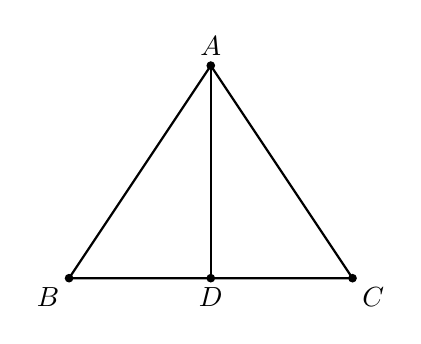
\begin{tikzpicture}[>=latex, scale=0.9]
  \coordinate (A) at (2.0,3.0);
  \coordinate (B) at (0,0);
  \coordinate (C) at (4.0,0);
  \coordinate (D) at (2.0,0);

  \draw[thick] (A) -- (B) -- (C) -- cycle;
  \draw[thick] (A) -- (D);
  \filldraw (A) circle (1.5pt) node[above] {$A$};
  \filldraw (B) circle (1.5pt) node[below left] {$B$};
  \filldraw (C) circle (1.5pt) node[below right] {$C$};
  \filldraw (D) circle (1.5pt) node[below] {$D$};
\end{tikzpicture}
\caption{等腰三角形性質}
\label{fig:b3-a1-17}
\end{figure}

\subsection*{習題 3}
\begin{enumerate}[1., leftmargin=2em]
  \item 等腰三角形頂角平分線平分對邊。
  \item 等腰三角形兩腰上中線必相等。
  \item 三角形中線若垂直底邊，則三角形必等腰。
  \item 二全等三角形的相當中線必相等。
\end{enumerate}
試證之。

% ==========================================
% § 4 平行線與內角和定理
% ==========================================
\subsection*{\S 4\quad 平行線與內角和定理}
\addcontentsline{toc}{subsection}{\S 4\quad 平行線與內角和定理}
\label{sec:b3_a1_4}

\subsubsection*{甲、首先，讓我們用基本性質 $\mathrm{III}_c$ 和 $\mathrm{I}_a$ 來證明下述定理。}

\noindent\textbf{定理 1}\quad 設 $l_1, l_2, l_3$ 是平面 $P$ 上的三條相異直線，$l_3$ 分別交 $l_1, l_2$ 於 $A, B$ 點（如圖 \ref{fig:b3-a1-18}）。若 $\angle 1 = \angle 2$，則直線 $l_1, l_2$ 不相交。

\begin{figure}[H]
\centering
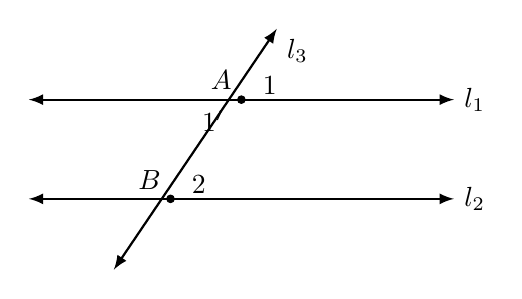
\begin{tikzpicture}[>=latex, scale=0.9]
  \draw[<->, thick] (-2,1.2) -- (4,1.2) node[right] {$l_1$};
  \draw[<->, thick] (-2,-0.2) -- (4,-0.2) node[right] {$l_2$};
  \draw[<->, thick] (-0.8,-1.2) -- (1.5,2.2) node[below right] {$l_3$};

  \coordinate (A) at (1.0,1.2);
  \coordinate (B) at (0.0,-0.2);
  \filldraw (A) circle (1.5pt) node[above left] {$A$};
  \filldraw (B) circle (1.5pt) node[above left] {$B$};

  \node at (1.4,1.4) {$1$};
  \node at (0.6,0.9) {$1'$};
  \node at (0.4,0.0) {$2$};
\end{tikzpicture}
\caption{內錯角相等則兩直線不相交}
\label{fig:b3-a1-18}
\end{figure}

\noindent【證明】\quad 我們將證明「$l_1, l_2$ 相交」這件事是不可能的，因為它會和性質 $\mathrm{I}_a$ 矛盾，這就是歸謬法。

假設 $l_1, l_2$ 相交於一點 $C$，在 $l_1$ 上 $A$ 的另一側取一點 $C'$，使得 $\overline{BC} = \overline{AC'}$（由性質 $\mathrm{III}_a$ 知道這樣的 $C'$ 唯一的存在）。

\begin{figure}[H]
\centering
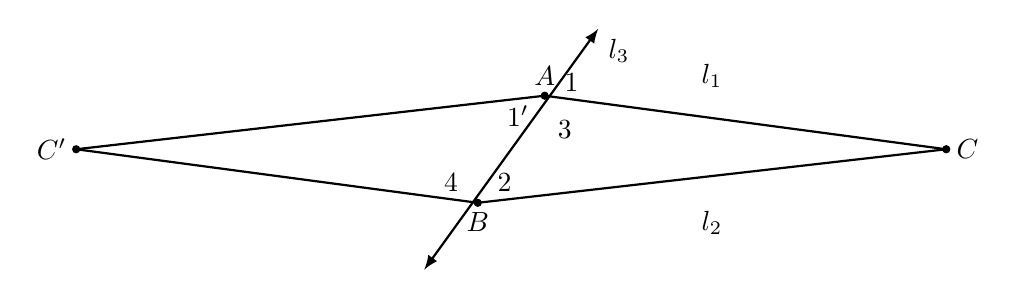
\begin{tikzpicture}[>=latex, scale=0.85]
  \coordinate (A) at (1.0,0.8);
  \coordinate (B) at (0.0,-0.8);
  \coordinate (C) at (7.0,0.0);
  \coordinate (Cp) at (-6.0,0.0);

  % 兩相交直線延伸
  \draw[thick] (Cp) -- (A) -- (C) node[right] {$C$};
  \draw[thick] (Cp) -- (B) -- (C);
  \node at (3.5,1.1) {$l_1$};
  \node at (3.5,-1.1) {$l_2$};

  % 截線 l3
  \draw[<->, thick] (-0.8,-1.8) -- (1.8,1.8) node[below right] {$l_3$};

  \filldraw (A) circle (1.5pt) node[above] {$A$};
  \filldraw (B) circle (1.5pt) node[below] {$B$};
  \filldraw (Cp) circle (1.5pt) node[left] {$C'$};
  \filldraw (C) circle (1.5pt);

  \node at (1.4,1.0) {$1$};
  \node at (0.6,0.5) {$1'$};
  \node at (1.3,0.3) {$3$};
  \node at (0.4,-0.5) {$2$};
  \node at (-0.4,-0.5) {$4$};
\end{tikzpicture}
\caption{定理 1 之反證法}
\label{fig:b3-a1-19}
\end{figure}

則如圖 \ref{fig:b3-a1-19} 所示，$\triangle BAC'$ 和 $\triangle ABC$ 對應地有下列關係：
\[ \angle A = \angle 1' = \angle 1 = \angle 2 = \angle B \quad \text{（對頂角相等及假設）} \]
\[ \overline{AB} = \overline{BA}, \quad \overline{AC'} = \overline{BC} \quad \text{（取 $C'$ 的條件）} \]
所以由性質 $\mathrm{III}_c$ 可知 $\triangle BAC'$ 和 $\triangle ABC$ 全等，故有
\[ \angle ABC' = \angle BAC \quad \text{（當然也有 $\angle C = \angle C', \overline{BC'} = \overline{AC}$）} \]
但是 $\angle 1' + \angle BAC = \text{平角}$，所以 $\angle C'BC = \angle 2 + \angle ABC'$ 也是一個平角，換句話說，$C', B, C$ 這三點在一直線上（即 $l_2$）這也就是說 $l_1, l_2$ 至少相交於 $C$ 與 $C'$ 這兩點，這顯然和性質 $\mathrm{I}_a$ 相矛盾，而這矛盾說明了「$l_1, l_2$ 相交」這個假設是不可能成立的，所以 $l_1$ 與 $l_2$ 只好不相交。

設 $l_2$ 是平面 $P$ 上的一直線，$A$ 是 $P$ 上不在直線 $l_2$ 上的一點，任取 $l_2$ 上一點 $B$，連結 $AB$ 得直線 $l_3$ 過 $A$ 點取直線 $l_1$，使得 $\angle 1 = \angle 2$（如圖 \ref{fig:b3-a1-20}）（根據 $\mathrm{III}_b$，這樣的直線 $l_1$ 一定存在）則由上面的證明得知 $l_1, l_2$ 不相交。

\begin{figure}[H]
\centering
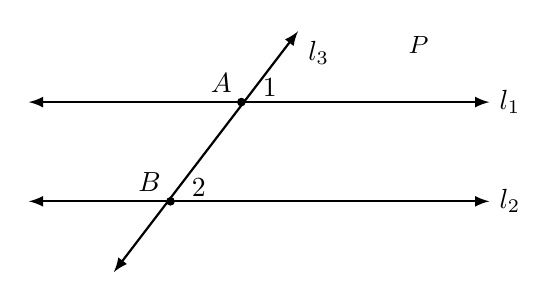
\begin{tikzpicture}[>=latex, scale=0.9]
  \draw[<->, thick] (-2,1.2) -- (4.5,1.2) node[right] {$l_1$};
  \draw[<->, thick] (-2,-0.2) -- (4.5,-0.2) node[right] {$l_2$};
  \draw[<->, thick] (-0.8,-1.2) -- (1.8,2.2) node[below right] {$l_3$};

  \coordinate (A) at (1.0,1.2);
  \coordinate (B) at (0.0,-0.2);
  \filldraw (A) circle (1.5pt) node[above left] {$A$};
  \filldraw (B) circle (1.5pt) node[above left] {$B$};

  \node at (1.4,1.4) {$1$};
  \node at (0.4,0.0) {$2$};
  \node at (3.5,2.0) {\small $P$};
\end{tikzpicture}
\caption{平行線之存在性}
\label{fig:b3-a1-20}
\end{figure}

在平面 $P$ 上，是不是還有其他過 $A$ 點而和 $l_2$ 不相交的直線呢？這是一個很值得研討的問題。

\subsubsection*{乙、在 \S 1-2 中我們提到一個極有意思的經驗性質\phantomsection\label{note:b3-a1-p273-sec}\footnote{【原書註記/校訂】：原書印作「在 \S 1-2 中我們提到一個極有意思的經驗性質」，實指第一冊第一章引言或第三冊第一章 § 1-1～§ 1-2 高斯測量三山峰三角形內角和之歷史背景．正文照原刊字樣錄入．}，即：}

\begin{quote}
  「任何三角形的內角和為一平角。」
\end{quote}
當然，任何這種經驗性的事實有賴於「度量」所以我們只能說，在儘可能精確的測量的「誤差範圍之內」，上述結果是對的，在理論上，「上述結果是不是絕對的成立？」是無法由實驗或測量去解答的，而從實用的眼光來看，既然在儘可能精確的測量下，上述結果在「誤差範圍之內」都是成立的，那我們當然可以假設「任何三角形的內角和為一平角」是絕對的成立，這樣在很多問題的討論和計算上可以簡便得多。

\noindent\textbf{基本性質 $\mathrm{IV}'$：}任意三角形的三內角和為一平角。

\noindent 性質 $\mathrm{IV}'$：可以用下述性質 $\mathrm{IV}$ 取代：

\noindent\textbf{基本性質 $\mathrm{IV}$。}在同一平面上，過定直線 $l$ 外一點 $A$，只有一直線與原直線 $l$ 不相交。

定理 1 說明了過 $A$ 點至少有一直線和 $l$ 不相交，如圖 18 中，取 $l = l_2$ 則 $l_1$ 即為如此之直線。基本性質 $\mathrm{IV}$ 說明 $l_1$ 是唯一的。這樣我們可以有下述定義。

\noindent\textbf{定義：}過線 $l$ 外一點 $A$，與 $l$ 不相交的直線，稱為過 $A$ 點 $l$ 的平行線。

此後將用 $l \parallel l'$ 表示 $l$ 與 $l'$ 互相平行（注意 $l$ 與 $l'$ 平行，即為 $l'$ 與 $l$ 平行）。

\subsection*{習題 4}

\noindent\textbf{三線八角：}兩直線同另一直線相交，所成的八個角可兩兩定名如下：

\begin{figure}[H]
\centering
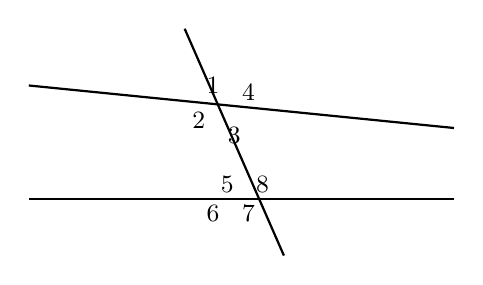
\begin{tikzpicture}[>=latex, scale=0.9]
  \draw[thick] (-2,1.2) -- (4,0.6);
  \draw[thick] (-2,-0.4) -- (4,-0.4);
  \draw[thick] (0.2,2.0) -- (1.6,-1.2);

  % 上交點
  \node at (0.6,1.2) {\small $1$};
  \node at (1.1,1.1) {\small $4$};
  \node at (0.4,0.7) {\small $2$};
  \node at (0.9,0.5) {\small $3$};

  % 下交點
  \node at (0.8,-0.2) {\small $5$};
  \node at (1.3,-0.2) {\small $8$};
  \node at (0.6,-0.6) {\small $6$};
  \node at (1.1,-0.6) {\small $7$};
\end{tikzpicture}
\caption{三線八角}
\label{fig:b3-a1-21}
\end{figure}

\begin{itemize}[leftmargin=2em]
  \item $\angle 1$ 與 $\angle 3, \angle 2$ 與 $\angle 4, \angle 5$ 與 $\angle 7, \angle 6$ 與 $\angle 8$ 互稱\textbf{對頂角}。
  \item $\angle 1$ 與 $\angle 5, \angle 4$ 與 $\angle 8, \angle 2$ 與 $\angle 6, \angle 3$ 與 $\angle 7$ 互稱\textbf{同位角}。（如圖 18 中之 $\angle 1 = \angle 2$ 亦是）
  \item $\angle 3$ 與 $\angle 5, \angle 2$ 與 $\angle 8$ 互稱\textbf{內錯角}。
  \item $\angle 1$ 與 $\angle 7, \angle 4$ 與 $\angle 6$ 互稱\textbf{外錯角}。
  \item $\angle 1$ 與 $\angle 6, \angle 4$ 與 $\angle 7$ 互稱\textbf{同側外角}。
  \item $\angle 2$ 與 $\angle 5, \angle 3$ 與 $\angle 8$ 互稱\textbf{同側內角}。
\end{itemize}

\begin{enumerate}[1., leftmargin=2em]
  \item 試證：
  \begin{enumerate}[(i)]
    \item 平行線之內錯角相等。
    \item 平行線之外錯角相等。
    \item 平行線之同側內角互補。
    \item 平行線之同側外角互補。
    \item 平行線之同位角相等。
  \end{enumerate}
  \item 試將題 1 中諸命題之逆命題寫出，並證明其亦真。
  \item 試證：兩直線若同平行於另一直線，則此二直線必平行。
\end{enumerate}

% ==========================================
% § 5 阿基米德性質與空間的完全性
% ==========================================
\subsection*{\S 5\quad 阿基米德性質與空間的完全性}
\addcontentsline{toc}{subsection}{\S 5\quad 阿基米德性質與空間的完全性}
\label{sec:b3_a1_5}

在第二冊第三章討論實數的次序與極限觀念時，我們已經說明了直線與實數之間的密切關係——直線的座標化。現在我們要把實數的阿基米德性質與完備性（參看第二冊第三章）用幾何觀念來敘述。

在正式開始之前，讓我們來看一下下面的說明：

假設我們要用一根尺去量線段 $\overline{AC}$ 長，當然我們先連直線 $\overline{AC}$，然後用尺自 $A$ 點向 $C$ 量。

$\overline{AC}$ 之長當然不一定正好等於幾公尺，一般的情形下，總是得一個像 5 公尺太少，6 公尺太多的情形。「公尺」當然是一個任意給定的單位，我們也可以用公寸，公丈，公分，英吋等任何單位去量，重要的是：不論我們用甚麼單位去量，我們早晚可以量出「$\overline{AC}$ 最多幾公尺」，「$\overline{AC}$ 最多幾吋」等結果，因為即使你用公厘做單位，自 $A$ 點一公厘一公厘地向 $C$ 量去，早晚你總可以超過 $C$ 點。

上面一段話用較嚴密的文字來說，便是：

\noindent\textbf{基本性質 $\mathrm{V}_a$（阿基米德性質）：}對於直線 $l$ 上 $A$ 點的同側的任給兩點 $B$ 與 $C$，必定存在一足夠大的正整數 $n$ 和位於 $A$ 點同側的一點 $B_n$，使得
\[ \overline{AB_n} = n \cdot \overline{AB} \quad \text{而且 $C$ 點位於 $A$ 與 $B_n$ 之間。} \]
亦即存在順序排列的 $A, B_1, B_2, B_3, \dots, B_n$，使得
\[ \overline{AB_1} = \overline{B_1B_2} = \overline{B_2B_3} = \dots = \overline{B_{n-1}B_n} \quad \text{而 $C$ 點位於 $A$ 與 $B_n$ 之間。} \]

\begin{figure}[H]
\centering
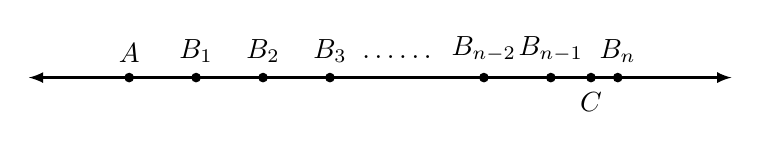
\begin{tikzpicture}[>=latex, scale=0.85]
  \draw[<->, thick] (-1,0) -- (9.5,0);
  \filldraw (0.5,0) circle (1.8pt) node[above=2pt] {$A$};
  \filldraw (1.5,0) circle (1.8pt) node[above=2pt] {$B_1$};
  \filldraw (2.5,0) circle (1.8pt) node[above=2pt] {$B_2$};
  \filldraw (3.5,0) circle (1.8pt) node[above=2pt] {$B_3$};
  \node at (4.5,0.3) {$\dots\dots$};
  \filldraw (5.8,0) circle (1.8pt) node[above=2pt] {$B_{n-2}$};
  \filldraw (6.8,0) circle (1.8pt) node[above=2pt] {$B_{n-1}$};
  \filldraw (7.8,0) circle (1.8pt) node[above=2pt] {$B_n$};
  \filldraw (7.4,0) circle (1.8pt) node[below=2pt] {$C$};
\end{tikzpicture}
\caption{阿基米德性質幾何示意圖}
\label{fig:b3-a1-22}
\end{figure}

在第二冊第三章中，我們已講過什麼叫做數列 $\langle a_n \mid n=1,2,3\dots \rangle$ 的極限，大體說來，如果 $a$ 是 $a_n$ 的極限，意思就是說在 $n$ 很大時，$a_n$ 的值和 $a$ 非常接近，如果我們把「$n$ 很大」和「非常接近」說清楚，那便是：對於任何正數 $\delta > 0$；如果我們都能找到一個數 $N$（$N$ 的大小當然可能被 $\delta$ 決定），而只要在 $n > N$ 時，恆有 $|a_n - a| < \delta$，那麼 $a$ 這個數便是數列 $\langle a_n \mid n=1,2,\dots \rangle$ 的極限值，例如我們知道 $\frac{1}{n} \to 0$，這是因為不論取得多麼小（如一兆分之一），我們總可以找到一個 $N$（例如一兆），而只要 $n > N$（= 一兆）時，我們總有
\[ \left| \frac{1}{n} - 0 \right| = \frac{1}{n} < \frac{1}{N} = \text{一兆分之一} = \delta \]
的緣故。

我們知道實數又可以看成數線上的點，因此數列 $\langle a_n \mid n=1,2,\dots \rangle$ 也可看成是直線上的\phantomsection\label{note:b3-a1-p276-ten}\footnote{【原書註記/校訂】：原書印作「直線上的十個點列」，依前後文理實指「一個點列」，字模「一」與「十」印刷誤植．正文照原刊字樣錄入．}十個點列，數列既然可以有極限的定義，做一個翻譯，用來定義直線上一點列的極限。

\noindent\textbf{定義}\quad 設 $\langle A_n \mid n=1,2,\dots \rangle$ 是直線 $l$ 上的「點列」，$B$ 是直線 $l$ 上的一個定點。假如對於任給正數 $\delta > 0$，皆存在一個夠大的正整數 $N$，使得
\begin{quote}
  對於任何 $n > N$，皆有 $\overline{BA_n}$ 的長度 $< \delta$
\end{quote}
則稱 $B$ 點為點列 $\langle A_n \rangle$ 的極限點。以符號
\[ \lim_{n \to \infty} A_n = B \]
表示，讀做 $B$ 點是 $\langle A_n \rangle$ 的極限點。

從這個定義，我們也可以體會到所謂 $\lim_{n \to \infty} A_n = B$ 的直觀幾何意義，簡單地說，便是 $n$ 很大時，$A_n$ 應該和 $B$ 很近。我們又可以反過來看這一個定義：

如果有一個 $B$ 點，而我們以 $B$ 為中點，向左、右距離為 $\delta$ 的地方各作一條防線，得線段 $\overline{B_1B_2}$ 如圖 \ref{fig:b3-a1-23}。

\begin{figure}[H]
\centering
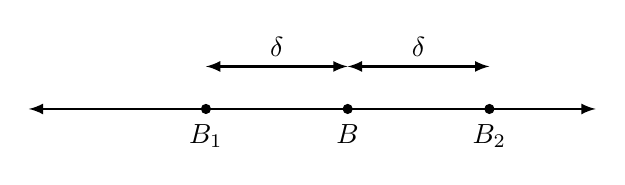
\begin{tikzpicture}[>=latex, scale=0.9]
  \draw[<->, thick] (-1,0) -- (7,0);
  \filldraw (1.5,0) circle (1.8pt) node[below=2pt] {$B_1$};
  \filldraw (3.5,0) circle (1.8pt) node[below=2pt] {$B$};
  \filldraw (5.5,0) circle (1.8pt) node[below=2pt] {$B_2$};

  \draw[<->, thick] (1.5,0.6) -- (3.5,0.6) node[midway, above] {$\delta$};
  \draw[<->, thick] (3.5,0.6) -- (5.5,0.6) node[midway, above] {$\delta$};
\end{tikzpicture}
\caption{極限點之幾何鄰域}
\label{fig:b3-a1-23}
\end{figure}

點列 $A_1, A_2, A_3 \dots$ 當然可能有無限多個點，如果這無數多個點裏，最多只有有限個點（不論是幾個，只要是有限個如 0 個、500 個、一兆個等），可能落在 $\overline{B_1B_2}$ 外面，而以上的要求又對所有的 $\delta$（不論多少，只要是正的！）都成立的話，那麼 $B$ 點就是點列 $A_n$ 的極限。

我們知道，任一個數列 $\langle a_n \mid n=1,2,\dots \rangle$ 不一定有極限，同樣地，並不是所有的點列都有極限。

實數系的性質往往都可以輕易地翻譯成直線上點的性質。同學們請想一想，下面的性質是從那些實數的性質翻譯來的。

\noindent\textbf{基本性質 $\mathrm{V}_b$（直線的完備性）：}設直線 $l$ 上的兩個點列 $\langle A_n \rangle$ 和 $\langle C_n \rangle$ 滿足下列性質：
\begin{enumerate}[(i), leftmargin=2.5em]
  \item 對任何正整數 $n, m$ 皆有 $A_n$ 位於 $A_{n-1}, C_m$ 之間，$C_m$ 位於 $A_n, C_{m-1}$ 之間（如圖 \ref{fig:b3-a1-24} 所示）。
  \item $\overline{A_nC_n}$ 的長度趨於 0 為極限。
\end{enumerate}
則必存在有直線 $l$ 上的一點 $B$，使得對於任何正整數 $n$，$B$ 點皆位於 $A_n, C_n$ 之間。

\begin{figure}[H]
\centering
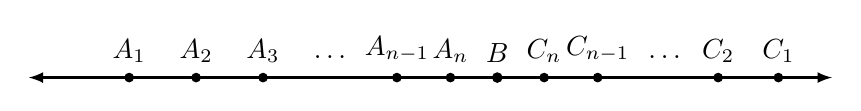
\begin{tikzpicture}[>=latex, scale=0.85]
  \draw[<->, thick] (-1,0) -- (11,0);
  \filldraw (0.5,0) circle (1.8pt) node[above=2pt] {$A_1$};
  \filldraw (1.5,0) circle (1.8pt) node[above=2pt] {$A_2$};
  \filldraw (2.5,0) circle (1.8pt) node[above=2pt] {$A_3$};
  \node at (3.5,0.3) {$\dots$};
  \filldraw (4.5,0) circle (1.8pt) node[above=2pt] {$A_{n-1}$};
  \filldraw (5.3,0) circle (1.8pt) node[above=2pt] {$A_n$};
  \filldraw (6.0,0) circle (2.0pt) node[above=2pt] {$B$};
  \filldraw (6.7,0) circle (1.8pt) node[above=2pt] {$C_n$};
  \filldraw (7.5,0) circle (1.8pt) node[above=2pt] {$C_{n-1}$};
  \node at (8.5,0.3) {$\dots$};
  \filldraw (9.3,0) circle (1.8pt) node[above=2pt] {$C_2$};
  \filldraw (10.2,0) circle (1.8pt) node[above=2pt] {$C_1$};
\end{tikzpicture}
\caption{直線完備性（區間套原理）}
\label{fig:b3-a1-24}
\end{figure}

$B$ 點也就是 $\langle A_n \rangle$ 和 $\langle C_n \rangle$ 的極限點：
\[ \lim_{n \to \infty} A_n = B = \lim_{n \to \infty} C_n \]

\subsection*{習題 5}
\begin{enumerate}[1., leftmargin=2em]
  \item 試寫出「點列」的定義。
  \item 試將相當於實數系完備性的第二形式之直線完備性寫出。
\end{enumerate}

\subsubsection*{綜合基本性質列表如下：}

\begin{itemize}[leftmargin=2em]
  \item[\textbf{基本性質 $\mathrm{I}$}]
  \begin{itemize}[leftmargin=2em]
    \item[$\mathrm{I}_a$：]任給空間相異兩點，有一條唯一的直線通過這兩點。
    \item[$\mathrm{I}_b$：]過平面上任意兩點的直線完全包含在該平面之內。
    \item[$\mathrm{I}_c$\phantomsection\label{note:b3-a1-p277-ic}\footnote{【原書註記/校訂】：原書此條印作「$\mathrm{I}$：過空間不共線三點」，漏印子標號「c」，前後文對應條目均為「$\mathrm{I}_c$」．正文予以校訂補齊．}：]過空間不共線三點，有一個唯一的平面。亦即，不共線三點決定一平面。
    \item[$\mathrm{I}_d$：]相異兩平面若相交，則交集為一直線。
    \item[$\mathrm{I}_e$：]一直線上至少有兩點；一平面上至少有不共線的三點；空間至少有不共面的四點。
  \end{itemize}

  \item[\textbf{基本性質 $\mathrm{II}$}]
  \begin{itemize}[leftmargin=2em]
    \item[$\mathrm{II}_a$：]對於直線上任給相異三點，其中必定有一個唯一的點位於其餘兩點之間。
    \item[$\mathrm{II}_b$：]「位於某兩點之間」這一關係與那兩點的順序無關。
    \item[$\mathrm{II}_c$：]對於直線上任給相異兩點 $A$ 與 $B$ 必存在位於其間的點，又存在另外兩點 $D$ 與 $E$，使得 $B$ 位於 $D$ 與 $A$ 之間，$A$ 位於 $B$ 與 $E$ 之間。
  \end{itemize}

  \item[\textbf{基本性質 $\mathrm{III}$}]
  \begin{itemize}[leftmargin=2em]
    \item[$\mathrm{III}_a$：]對於任給線段 $\overline{AB}$ 和過 $A'$ 點的直線 $l'$，在 $l'$ 上 $A'$ 點的兩側個別存在唯一的點 $B'$ 與 $B''$ 使得 $\overline{A'B'}$ 及 $\overline{A'B''}$ 與 $\overline{AB}$ 全等。
    \item[$\mathrm{III}_b$\phantomsection\label{note:b3-a1-p278-l3p}\footnote{【原書註記/校訂】：原書此處印作「$l_2'$ 和 $l_3'$」，前文頁 271 正式條文及插圖均為「$l_2'$ 和 $l_2''$」．正文照原刊字樣錄入．}：]對於任給 $A$ 點的角 $(l_1, l_2)$ 及任給過另一點 $A'$ 點的平面 $P'$ 和 $P'$ 上過 $A'$ 的一有向直線 $l_1'$，在 $P'$ 上直線 $l_1'$ 的兩側分別存在唯一的一過 $A'$ 點有向直線 $l_2'$ 和 $l_3'$，使得角 $(l_1', l_2')$ 及角 $(l_1', l_3')$ 和 $(l_1, l_2)$ 的角度相等。
    \item[$\mathrm{III}_c$：]兩三角形若有兩邊及一夾角相等則兩形全等。
  \end{itemize}

  \item[\textbf{基本性質 $\mathrm{IV}$}]
  \begin{itemize}[leftmargin=2em]
    \item[$\mathrm{IV}$：]在同一平面上，過直線 $l$ 外一點 $A$ 只有一條直線，它和原直線 $l$ 不相交。
    \item[$\mathrm{IV}'$：]任何三角形的三內角和為一平角。
  \end{itemize}

  \item[\textbf{基本性質 $\mathrm{V}$}]
  \begin{itemize}[leftmargin=2em]
    \item[$\mathrm{V}_a$：]（阿基米德性質）：對於直線 $l$ 上 $A$ 點的同側的任給兩點 $B$ 與 $C$。必定存在一足夠大的正整數 $n$ 和位於 $A$ 點同側的一點 $B_n$，使得 $\overline{AB_n} = n \cdot \overline{AB}$，而且 $C$ 點位於 $A$ 與 $B_n$ 之間。
    \item[$\mathrm{V}_b$：]（直線的完備性）：直線 $l$ 上二點列 $\langle A_n \rangle$ 和 $\langle C_n \rangle$ 若滿足下列性質：
    \begin{enumerate}[(i)]
      \item 對任何正整數 $n, m$ 皆有 $A_n$ 位於 $A_{n-1}, C_m$ 之間，$C_m$ 位於 $A_n, C_{m-1}$ 之間。
      \item $\overline{A_nC_n}$ 的長度趨於 0。
    \end{enumerate}
    則其上必存在一點 $B$，使得對所有 $n$，$B$ 點位於 $A_n, C_n$ 之間。
  \end{itemize}
\end{itemize}

% ==========================================
% § 6 性質 IV 和性質 IV' 的等價性證明
% ==========================================
\subsection*{\S 6\quad 性質 $\mathrm{IV}$ 和性質 $\mathrm{IV}'$ 的等價性證明}
\addcontentsline{toc}{subsection}{\S 6\quad 性質 $\mathrm{IV}$ 和性質 $\mathrm{IV}'$ 的等價性證明}
\label{sec:b3_a1_6}

最後我們要證明性質 $\mathrm{IV}$ 和性質 $\mathrm{IV}'$ 是等價的，也就是說：
\begin{center}
  從性質 $\mathrm{IV}$ 出發可以推演得性質 $\mathrm{IV}'$；而\\
  從性質 $\mathrm{IV}'$ 出發也可以推演得性質 $\mathrm{IV}$。
\end{center}
當然，在推演的過程中，我們得要用到基本性質 $\mathrm{I}, \mathrm{II}, \mathrm{III}, \mathrm{V}$ 所以嚴格的說來，應該是要證明：
\begin{quote}
  「體系 $\mathrm{I}, \mathrm{II}, \mathrm{III}, \mathrm{IV}, \mathrm{V}$」和「體系 $\mathrm{I}, \mathrm{II}, \mathrm{III}, \mathrm{IV}', \mathrm{V}$」在邏輯上是等價的。
\end{quote}

\subsubsection*{由 $\mathrm{IV}$ 去證明 $\mathrm{IV}'$：}

我們將由歸謬法證明三角形之內角和不是一平角是不可能的，假如存在一 $\triangle ABC$ 其三內角和不是一個平角，如圖 \ref{fig:b3-a1-25} 所示，我們過 $A$ 點作直線 $l_1$ 使得 $\angle 1' = \angle 1$；作直線 $l_2$ 使得 $\angle 2' = \angle 2$，再者 $\angle 3'$ 和 $\angle 3$ 是對頂角，所以顯然有 $\angle 3' = \angle 3$。故
\[ \angle 1' + \angle 3' + \angle 2' = \angle 1 + \angle 3 + \angle 2 \neq \text{一平角} \]
所以 $l_1$ 和 $l_2$ 是不同的二條直線。

而由定理 1 得知 $l_1, l_2$ 都和 $l$ 不相交，這顯然和性質 $\mathrm{IV}$ 相矛盾，所以假如性質 $\mathrm{IV}$ 成立，則性質 $\mathrm{IV}'$ 也隨而成立。

\begin{figure}[H]
\centering
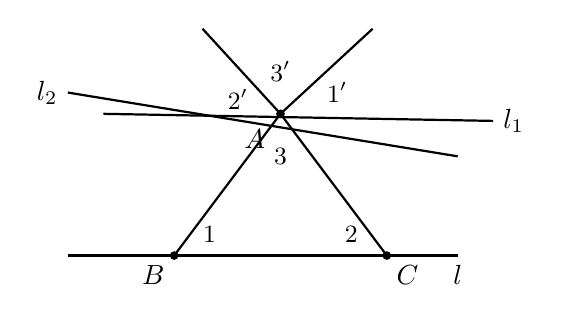
\begin{tikzpicture}[>=latex, scale=0.9]
  \coordinate (A) at (2.5,2.0);
  \coordinate (B) at (1.0,0);
  \coordinate (C) at (4.0,0);

  \draw[thick] (-0.5,0) -- (5.0,0);
  \node[below] at (5.0,0) {$l$};
  \draw[thick] (A) -- (B) -- (C) -- cycle;

  \filldraw (A) circle (1.5pt) node[below left=2pt] {$A$};
  \filldraw (B) circle (1.5pt) node[below left] {$B$};
  \filldraw (C) circle (1.5pt) node[below right] {$C$};

  % 直線 l1 (過 A 使 1' = 1)
  \draw[thick] (0.0,2.0) -- (5.5,1.9) node[right] {$l_1$};
  % 直線 l2 (過 A 使 2' = 2)
  \draw[thick] (-0.5,2.3) node[left] {$l_2$} -- (5.0,1.4);

  % 頂角處射線及角標記
  \draw[thick] (A) -- (3.8,3.2);
  \draw[thick] (A) -- (1.4,3.2);

  \node at (1.5,0.3) {\small $1$};
  \node at (3.5,0.3) {\small $2$};
  \node at (2.5,1.4) {\small $3$};

  \node at (3.3,2.3) {\small $1'$};
  \node at (2.5,2.6) {\small $3'$};
  \node at (1.9,2.2) {\small $2'$};
\end{tikzpicture}
\caption{由 $\mathrm{IV}$ 證 $\mathrm{IV}'$}
\label{fig:b3-a1-25}
\end{figure}

\subsubsection*{由 $\mathrm{IV}'$ 去證明 $\mathrm{IV}$：}

如圖 \ref{fig:b3-a1-26} 所示，直線 $l$ 和 $A$ 是平面 $P$ 上的任給直線和線外一點，任取 $l$ 上一點 $B$，連結直線 $AB$ 過點 $A$ 作直線 $l'$ 使得 $\angle 1 = \angle 1'$。如圖 \ref{fig:b3-a1-26} 所示，在 $l$ 上取 $C_1$ 點使得 $\overline{BA} = \overline{BC_1}$，連結 $A, C_1$ 得直線 $l_1$，然後再在 $l$ 上取 $C_2$ 點使得 $\overline{C_1A} = \overline{C_1C_2}$，連結 $A, C_2$ 得直線 $l_2$ 以此逐步在 $l$ 上取 $C_n$ 點，使得 $\overline{C_{n-1}A} = \overline{C_{n-1}C_n}$，連結 $A, C_n$ 得直線 $l_n$，由上面的條件可知 $\triangle ABC_1, \triangle AC_1C_2, \dots, \triangle AC_{n-1}C_n, \dots$ 都是等腰三角形，所以其底角相等。

\begin{figure}[H]
\centering
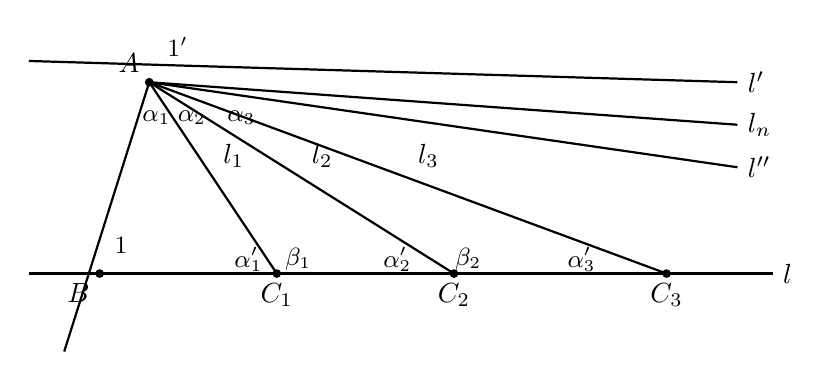
\begin{tikzpicture}[>=latex, scale=0.9]
  \coordinate (A) at (1.2,3.5);
  \coordinate (B) at (0.5,0.8);
  \coordinate (C1) at (3.0,0.8);
  \coordinate (C2) at (5.5,0.8);
  \coordinate (C3) at (8.5,0.8);

  % 基線 l
  \draw[thick] (-0.5,0.8) -- (10.0,0.8) node[right] {$l$};
  \filldraw (B) circle (1.5pt) node[below left] {$B$};
  \filldraw (C1) circle (1.5pt) node[below] {$C_1$};
  \filldraw (C2) circle (1.5pt) node[below] {$C_2$};
  \filldraw (C3) circle (1.5pt) node[below] {$C_3$};

  % 直線 AB
  \draw[thick] (0.0,-0.3) -- (A);
  \filldraw (A) circle (1.5pt) node[above left] {$A$};

  % 平行線 l'
  \draw[thick] (-0.5,3.8) -- (9.5,3.5) node[right] {$l'$};

  % 連線 AC1, AC2, AC3
  \draw[thick] (A) -- (C1) node[midway, above right] {$l_1$};
  \draw[thick] (A) -- (C2) node[midway, above right] {$l_2$};
  \draw[thick] (A) -- (C3) node[midway, above right] {$l_3$};

  % 其他射線 ln, l''
  \draw[thick] (A) -- (9.5,2.9) node[right] {$l_n$};
  \draw[thick] (A) -- (9.5,2.3) node[right] {$l''$};

  % 角標記
  \node at (0.8,1.2) {\small $1$};
  \node at (1.6,4.0) {\small $1'$};

  \node at (1.3,3.0) {\small $\alpha_1$};
  \node at (1.8,3.0) {\small $\alpha_2$};
  \node at (2.5,3.0) {\small $\alpha_3$};

  \node at (2.6,1.0) {\small $\alpha_1'$};
  \node at (3.3,1.0) {\small $\beta_1$};
  \node at (4.7,1.0) {\small $\alpha_2'$};
  \node at (5.7,1.0) {\small $\beta_2$};
  \node at (7.3,1.0) {\small $\alpha_3'$};
\end{tikzpicture}
\caption{由 $\mathrm{IV}'$ 證 $\mathrm{IV}$}
\label{fig:b3-a1-26}
\end{figure}

再由性質 $\mathrm{IV}'$ 可得
\begin{align*}
  &\angle 1 + \angle \alpha_1 + \angle \alpha_1' = 180^\circ \quad \text{及} \quad \angle \alpha_1 = \angle \alpha_1' \\
  \Longrightarrow\quad &\angle \alpha_1 = \angle \alpha_1' = \frac{1}{2}(180^\circ - \angle 1) \\[0.5em]
  &\angle \alpha_2 = \angle \alpha_2' \quad \text{及} \quad \angle \beta_1 + \angle \alpha_2 + \angle \alpha_2' = 180^\circ = \angle \beta_1 + \angle \alpha_1' \\
  \Longrightarrow\quad &\angle \alpha_2 = \angle \alpha_2' = \frac{1}{2}\angle \alpha_1' = \frac{1}{2}\angle \alpha_1 = \frac{1}{2^2}(180^\circ - \angle 1) \text{。}
\end{align*}
同理有
\begin{align*}
  &\angle \alpha_n = \angle \alpha_n' \quad \text{及} \quad \angle \beta_{n-1} + \angle \alpha_n + \angle \alpha_n' = 180^\circ = \angle \beta_{n-1} + \angle \alpha_{n-1} \\
  \Longrightarrow\quad &\angle \alpha_n = \angle \alpha_n' = \frac{1}{2}\angle \alpha_{n-1}' = \frac{1}{2}\angle \alpha_{n-1} = \frac{1}{2^n}(180^\circ - \angle 1)
\end{align*}
所以直線 $l_n$ 和 $l'$ 在 $A$ 點的夾角（$= \angle \alpha_n$）趨於 0 為極限，而直線 $l_n$ 和 $l$ 相交。

設 $l''$ 是任何一條過 $A$ 點異於 $l'$ 的直線，當 $n$ 相當大時，$(l', l_n)$ 的夾角就小於 $(l', l'')$ 的夾角（如圖 \ref{fig:b3-a1-26} 所示），但是 $l_n$ 和 $l$ 相交於 $C_n$ 點。所以 $l''$ 一定和 $l$ 交於 $\overline{BC_n}$ 之間的一點；這也就證明了任何過 $A$ 點異於 $l'$ 的直線皆和 $l$ 相交，亦即 $l'$ 是唯一的過 $A$ 點和 $l$ 不相交的直線。

故性質 $\mathrm{IV}$ 成立。
